\begin{savequote}[75mm]
“As always in life, people want a simple answer \. \. \. and it’s always wrong.”
\qauthor{Susan Greenfield}
\end{savequote}

\chapter{Fusion Gene Detection}\label{chapter:fusiongenes}
\setcounter{figure}{-1}
\setcounter{table}{-1}
\setcounter{section}{-1}

\begin{figure}[t!]
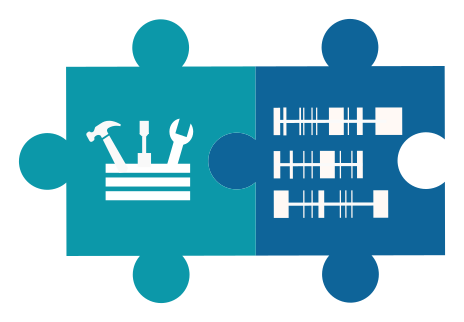
\includegraphics[height=10em]{frontmatter/images/chapter-header-fusion-tools.png}
\end{figure}
\setcounter{figure}{-1}
\setcounter{table}{-1}
\setcounter{section}{-1}


Structural variations are large-scale rearrangements of the genome. When these alterations occurr within genes, novel hybrid genes called \emph{fusion genes} may be formed. Accurate detection of SVs and resulting fusion genes are an informative in cancer research studies.

We created iFUSE, web-based application to visualize and explore structural variants, and identify and prioritize potential fusion genes within a sample. We subsequently used this tool to detect multiple fusions in VCaP cell line. Futhermore, we were discovered chromothirpsis on chromosome 5q of this sample, and used the Circos tool to visualize this in a single plot.

This chapter contains the following sub-chapters:

\begin{enumerate}[label=\ref{chapter:fusiongenes}.\arabic*]
\itemsep-0.5em
\setcounter{enumi}{-1}
\item \textbf{iFUSE:} integrated fusion gene explorer
\item Gene fusions by chromothripsis of chromosome 5q in the VCaP prostate cancer cell line
\end{enumerate}
